\chapter{Implementation and evaluation}
\label{chap:impl}

In this chapter the implementation of proposed method and results 
of numerical experiments are shown. Firstly, Section {\ref{sec:dual_arm_yumi}} 
contains information about chosen system and its properties. Then, in Section 
\ref{sec:frameworks} the discussion of used frameworks and utils is presented. 
Consequently, these tools are used in Section \ref{sec:impl_details} to show 
how the proposed algorithms can be implemented. Finally, Section 
\ref{sec:sim_results} contains results of numerical experiments with their 
evaluation.

\section{Dual-arm YuMi}
\label{sec:dual_arm_yumi}

To prove the workability of the suggested methodology the dual-arm YuMi 
manipulator is chosen, see Fig. \ref{fig:dual_arm_yumi}. It has 18 DoF, namely: 
7 rotation and 2 prismatic (fingers) joints per each arm. 

In simulation the total DoF was reduced to 14 by fixing end-effectors' fingers. 
Also for demonstration purposes the joint limits and body collisions were 
removed. Otherwise, their presence could influence on final results.

\begin{figure}[H]
    \centering
    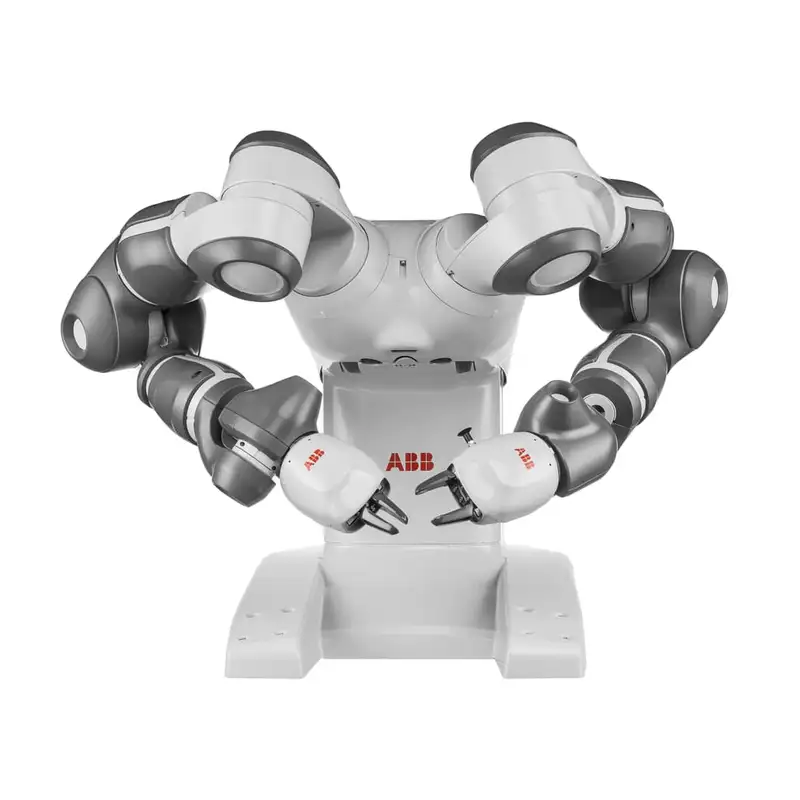
\includegraphics[scale=0.25]{figs/yumi.png}
    \caption{Dual-arm YuMi IRB 14000}
    \label{fig:dual_arm_yumi}
\end{figure}

The discussed manipulator was selected because there is URDF (Unified Robot 
Description Format) for it. However, there was no necessary representation for the 
chosen simulator. Thus, it was generated. Details is conducted later 
in Section \ref{sec:impl_details}.

\section{Frameworks}
\label{sec:frameworks}

For implementation the discussed algorithms C++ is used. Beyond of chosen language 
it is also necessary to select a simulator, a tool for computing dynamics, and 
library for solving the Gauss least constraint principle 
(\ref{eqn:least_act_principle_const}). In this section all of them is reviewed.

Firstly, let's discuss chosen simulator, MuJoCo \cite{MuJoCo}. It is general 
physical engine. In this study this framework is used to calculate system 
behavior under given Control. Also, it provides way to visualize robot. From 
control point of view MuJoCo is only needed to give $\mathbf{q}$ and $\mathbf{v}$ 
at each step. 

The system state is transferred to dynamic computing tool. This paper is utilizing 
Pinocchio \cite{Pinocchio} library. It is modern and efficient instrument for 
calculating kinematic and dynamic for given system. Notably, this frameworks 
supports the URDF, which is very convenient in the context of the selected system. 
Moreover, Pinocchio provides fast computational utils. Authors of tool give 
the following quantities, see Fig. \ref{fig:pin_speed}. For implementation this 
library is necessary to calculate Jacobians, attitudes of frames, and velocities.

\begin{figure}[H]
    \centering
    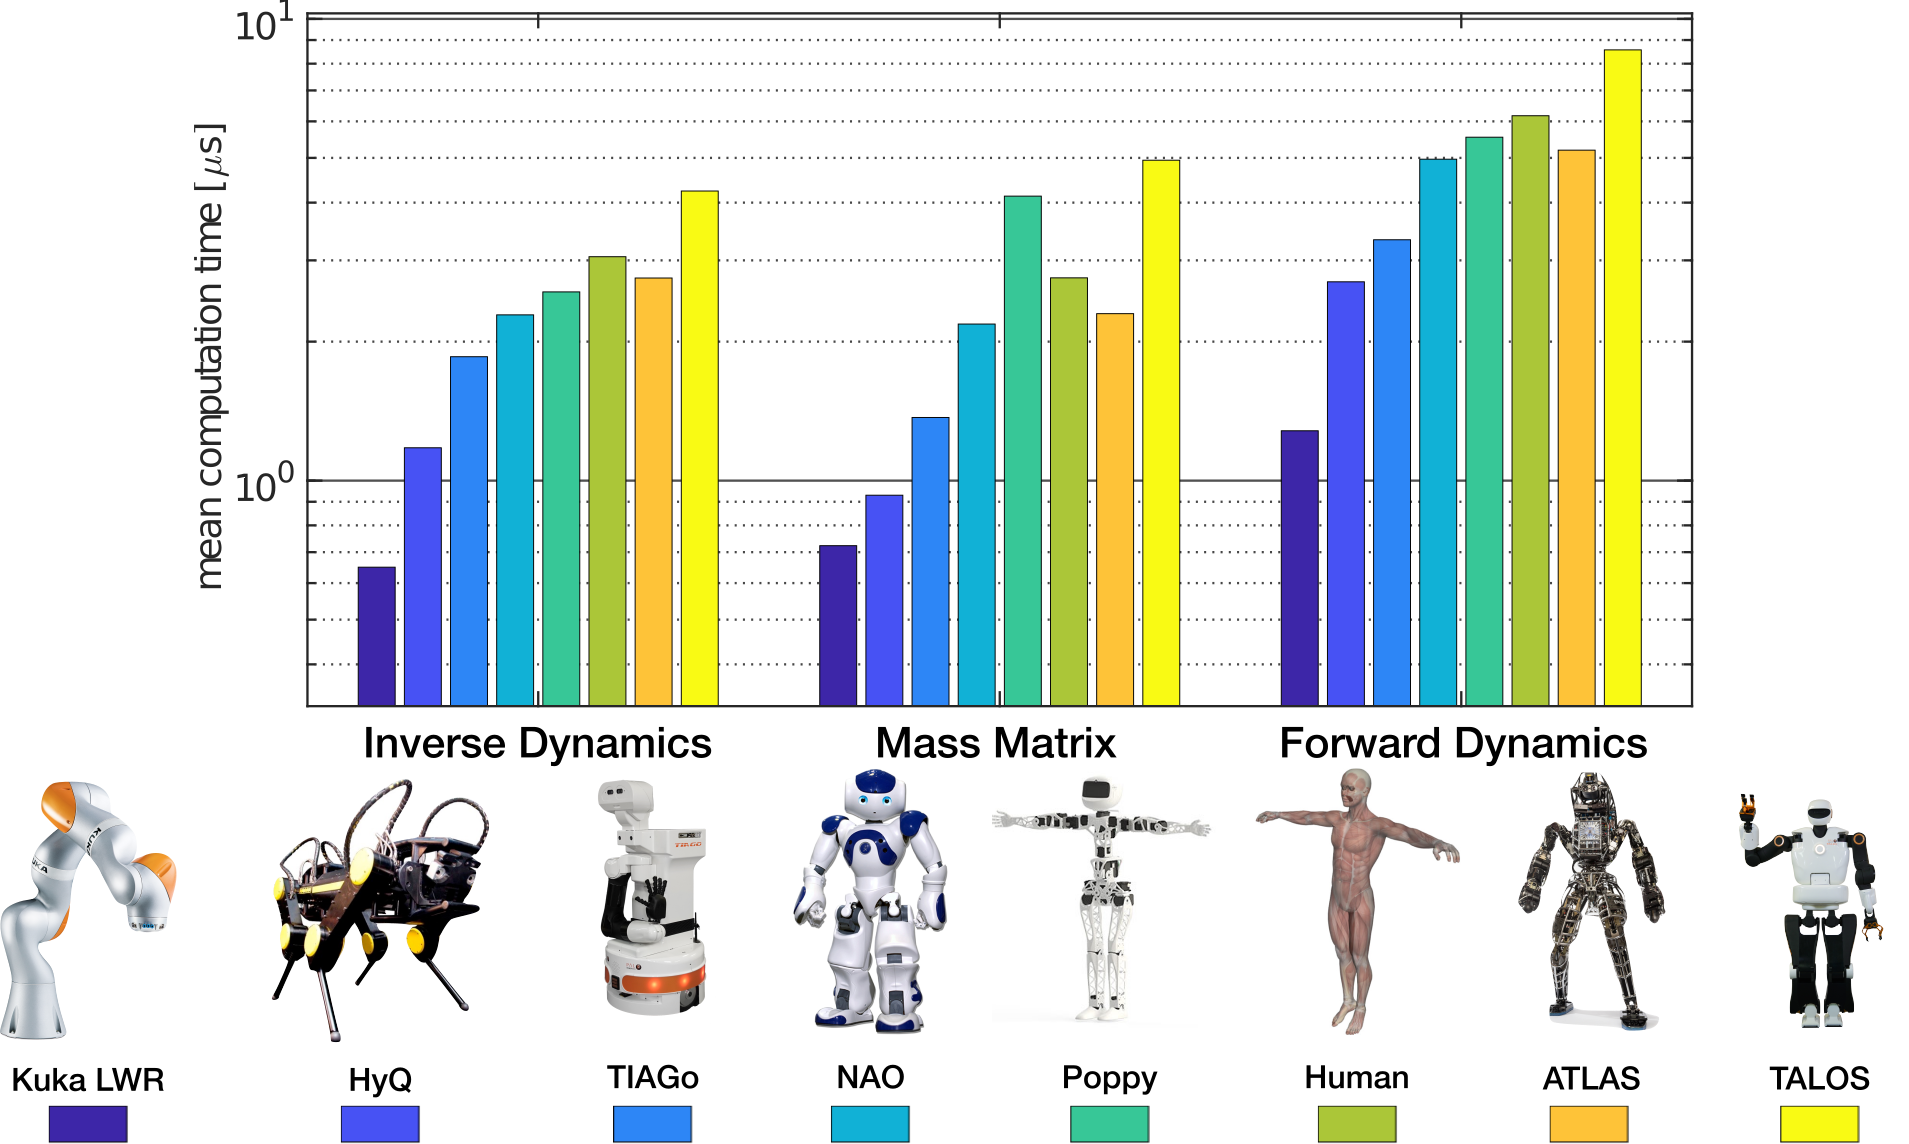
\includegraphics[scale=0.2]{figs/pin_speed.png}
    \caption{Pinocchio performance demonstration}
    \label{fig:pin_speed}
\end{figure}

Finally, the last needed element is optimization problem solver. In this paper 
ProxSuite \cite{ProxQP} is used for such purpose. The suggested methodology lies 
on quadratic problem. Authors of ProxSuite shows that their tool is fast of 
solving it. The mean computation time is 10 microseconds, see Fig. 1 in 
\cite{ProxQP}. Although, the discussed instrument is efficient but the problem 
(\ref{eqn:gauss_least_const_prior}) can be directly solved. Thus, it is needed 
to be reformulated. Further details is provided later in Section \ref{sec:impl_details}

\section{Implementation details}
\label{sec:impl_details}

This section contains details of implementation of the suggested methodology. It 
can be split into two parts, namely: computing $A$ and $\mathbf{b}$ with Pinocchio, 
and solving the problem (\ref{eqn:gauss_least_const_prior}) by ProxSuite. 
Remarkably, in this section there is no details about simulation and visualization 
because they described in MuJoCo documentation. However, it is necessary to 
mention that there is no YuMi representation for this simulator. Let's 
first discuss this moment.

The MuJoCo physical engine supports only specific XML description. It is usually 
called MJCF. For numerical experiment the total DoF was reduced to 14. Only rotation 
joints were remained. For demonstration purposes it is enough.

Now let's consider implementation of proposed algorithms 
\ref{alg:get_a_and_b}, \ref{alg:get_a_and_b_control_fixed}, and 
\ref{alg:get_a_and_b_control_rigid}. For all of them it is obligatory to compute 
Jacobians, attitude of frames, and velocities. Let's starts from system model 
and data definition:

\begin{lstlisting}[caption={Model and data}, label=snp:model_and_data]
namespace pin = pinocchio;
...
pin::Model m;
pin::urdf::buildModel("path/to/urdf", m);
pin::Data d(m);
\end{lstlisting}

Next it is necessary to compute forward kinematics for given model. As input this 
step requires generalized coordinates and velocities ($\mathbf{q}$ and 
$\mathbf{v}$). See below snippet:

\begin{lstlisting}[caption={Forward kinematics}, label=snp:forward_kin]
pin::forwardKinematics(m, d, q, v);
pin::computeJointJacobians(m, d, q);
pin::computeJointJacobiansTimeVariation(m, d, q, v);
pin::updateFramePlacements(m, d);
\end{lstlisting}

Now Jacobians, attitudes of frames, and velocities can be calculated. If $E$ is 
origin of some frame attached to system, then it has a special id in Pinocchio 
description. Let's call it \texttt{eIdx}. Thus, the code for Jacobians is

\begin{lstlisting}[caption={Jacobians}, label=snp:jacs]
using MatXd = Eigen::MatrixXd;
...
MatXd jac = MatXd::Zero(6, m.nv);
MatXd dJac = MatXd::Zero(6, m.nv);
pin::getFrameJacobian(m, d, eIdx, pin::LOCAL_WORLD_ALIGNED, jac);
pin::getFrameJacobianTimeVariation(m, d, eIdx, pin::LOCAL_WORLD_ALIGNED, dJac);
\end{lstlisting}

Here \texttt{jac} and \texttt{dJac} are Jacobian and its derivative over time 
respectively. It is important to mention that these quantities from 
$\mathbb{R}^{6 \times n_v}$. The first three rows are corresponding to 
classical linear velocity, $J_{E,v}$ or $\dot{J}_{E,v}$. The bottom three rows are 
angular part, $J_{E,\omega}$ or $\dot{J}_{E,\omega}$. All of them are expressed 
in the world coordinates.

For attitudes and velocities it is enough to execute

\begin{lstlisting}[caption={Attitudes of frames}, label=snp:atts_of_frames]
pin::Frame eFrame = m.frames[idx];
pin::FrameIndex pIdx = frame.parent;
pin::SE3 localToWorldY = pin::SE3::Identity();
localToWorldY.rotation(d.oMf[eIdx].rotation());
pin::SE3 eAtt = d.oMf[eIdx]; 
pin::Motion eVel = localToWorldY.act(frame.placement.actInv(d.v[pIdx]));
\end{lstlisting}

In snippet (\ref{snp:atts_of_frames}) \texttt{eAtt} and \texttt{eVel} are 
frame attitude and velocity respectively. \texttt{eVel} contains linear and 
angular part.

The last parts worth mentioning are the skew-symmetric operator ($[.]^{\wedge}$) 
and matrix logarithm ($\log (.)$). In Pinocchio they are \texttt{pin::skew} and 
\texttt{pin::log3} function respectively. Other mathematical operations are not 
worth to be explained due to their triviality. 

All snippets above are used for experiment. They can be found in the repository 
\textcolor{red}{REF TO REP}. However, for optimization and readability they 
are realized not in the same order. In the provided code algorithm 
\ref{alg:get_a_and_b} is demonstrated in \texttt{getConstraintsAffineDesc}, 
algorithm \ref{alg:get_a_and_b_control_fixed} is shown in \\
\texttt{getControlAffineDesc}, the last one \ref{alg:get_a_and_b_control_rigid} 
can be implemented by function \\ \texttt{getAffineDesc}.

Now let's discuss the transformation of equation 
(\ref{eqn:gauss_least_const_prior}) for ProxSuite framework. This library can 
handle quadratic problem of the following form

\begin{equation}
    \begin{aligned}
        \min_{\mathbf{x}} \quad & 
        \frac{1}{2} \mathbf{x}^T H \mathbf{x} + 
        \mathbf{g}^T \mathbf{x} \\
        \textrm{s.t.} \quad & A \mathbf{x} = \mathbf{b} \\
        & \mathbf{y}_l \leq C \mathbf{x} \leq \mathbf{y}_u  
    \end{aligned}
    \label{eqn:prox_qp_form}
\end{equation}

where $[.] \leq [.]$ is element-wise vector operator, $H \succeq 0$, and 
other quantities are arbitrary.

In case of the Gauss least constraint principle the last line of quadratic 
problem (\ref{eqn:prox_qp_form}) is unnecessary. Hence, it is enough 
to pen brackets of equation (\ref{eqn:gauss_least_const_prior}):

\begin{equation}
    \begin{aligned}
        \min_{\dot{\mathbf{v}}} \quad & 
        \frac{1}{2} \dot{\mathbf{v}}^T [M + \omega A_u^T A_u] \dot{\mathbf{v}} + 
        [-\mathbf{Q} - \omega A_u^T \mathbf{b}_u]^T \dot{\mathbf{v}} \\
        \textrm{s.t.} \quad & A_c \dot{\mathbf{v}} = \mathbf{b}_c
    \end{aligned}
    \label{eqn:gauss_least_const_to_prox_qp}
\end{equation}

The removing of unconstrained acceleration $\mathbf{a}$ is possible by equation 
(\ref{eqn:can_man_eqn_simple}). Thus, $H = M + \omega A_u^T A_u$ and 
$\mathbf{g} = -\mathbf{Q} - \omega A_u^T \mathbf{b}_u$. The problem 
(\ref{eqn:gauss_least_const_to_prox_qp}) is solvable by the following 
code

\begin{lstlisting}[caption={Quadratic problem solution}, label=snp:qp_sol]
namespace prox = proxsuite::proxqp;
...
prox::dense::QP<double> qp(m.nv, 6, 0);
qp.settings.eps_abs = eps_abs;
qp.settings.initial_guess = prox::InitialGuessStatus::NO_INITIAL_GUESS;
qp.settings.verbose = false;
qp.init(
    M + omega * Au.transpose() * Au,
    -Q - omega * Au.transpose() * bu,
    Ac, bc,
    proxsuite::nullopt, proxsuite::nullopt, proxsuite::nullopt
);
qp.solve();
\end{lstlisting}

After first computation it is recommended to use \\
\texttt{prox::InitialGuessStatus::WARM\_START} to speed up calculation. This 
flag enables initial guess taken from previous solution.

\section{Simulation results}
\label{sec:sim_results}

During the experiment the following presets for YuMi are following

\begin{longtable}{|p{.30\textwidth}|l|}
\hline
Quantity & Used in experiment \\ 
\hline
Frame $\mathcal{E}_1$ & Joint frame \texttt{yumi\_link\_7\_l} in URDF \\ 
\hdashline
Frame $\mathcal{E}_2$ & Joint frame \texttt{yumi\_link\_7\_r} in URDF \\ 
\hdashline
$T_{\mathcal{A}}^{\mathcal{B}}$ & 
$\begin{bmatrix}
    1 & 0 & 0 & 0 \\
    0 & 0 & 1 & -0.4 \\
    0 & -1 & 0 & 0.12 \\
    0 & 0 & 0 & 1  
\end{bmatrix}$ \\
\hdashline
Constraint $K_p$ & 1000 \\
\hdashline
Constraint $K_d$ & 33 \\ 
% \hline
Control $K_p$ & 500 \\ 
\hdashline
Control $K_d$ & 17 \\ 
\hdashline
$\omega$ from equation (\ref{eqn:gauss_least_const_prior}) & 50 \\ 
\hdashline
Desired law ($T_{\mathcal{W}}^{\mathcal{D}}$) of motion for $\mathcal{E}_1$ & 
$\begin{bmatrix}
    1 & 0 & 0 & 0.436763 + 0.12 \cdot \cos(1.5 t + \pi / 2) \\
    0 & 1 & 0 & 0.185684 \\
    0 & 0 & 1 & 0.512661 + 0.12 \cdot \sin(1.5 t + \pi / 2) \\
    0 & 0 & 0 & 1
\end{bmatrix}$ \\ 
\hdashline
Initial $\mathbf{q}$ & See in \textcolor{red}{REF TO REP} \\ 
\hdashline
Initial $\mathbf{v}$ & $\mathbf{0}$ \\ 
\hline
\end{longtable}

The initial $\mathbf{q}$ is around of ideal one that gives zero control and 
constraint error. Simulation shows the following behavior of generalized 
coordinates and velocities under proposed control, see Fig. \ref{fig:q_and_v_plot}

\begin{figure}[H]
    \centering
    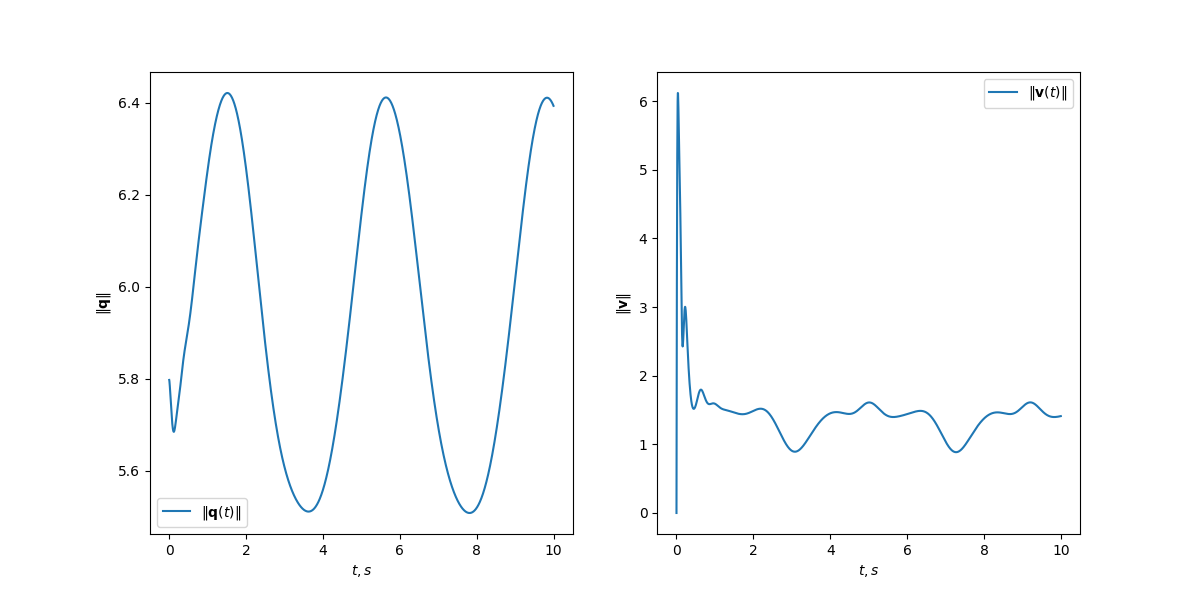
\includegraphics[scale=0.52]{figs/q_and_v_history.png}
    \caption{Experimental $\mathbf{q}$ and $\mathbf{v}$}
    \label{fig:q_and_v_plot}
\end{figure}

The plot of $\|\mathbf{q}\|$ and $\|\mathbf{v}\|$ over time demonstrates 
convergence to some periodical function. It can be explained by chosen 
desired law with period $4 \pi / 3$. Although, it is indirect proof of success, but 
the plot of positions shows stability of proposed methodology, see Fig. 
\ref{fig:poses_plot}. Subscript $s$ stands for $\mathcal{E}_1$ frame, 
and $e$ stands for $\mathcal{E}_2$.

\begin{figure}[H]
    \centering
    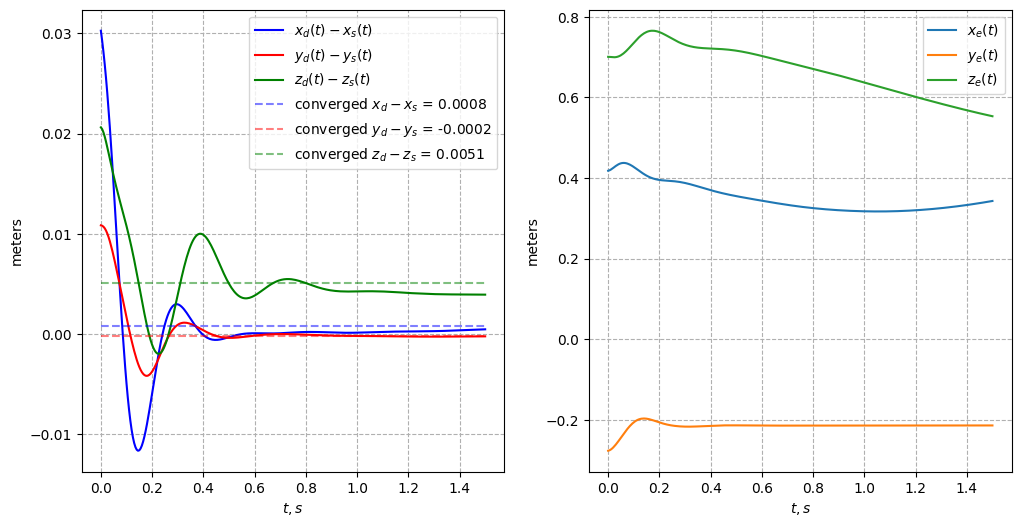
\includegraphics[scale=0.52]{figs/poses_history.png}
    \caption{Experimental frame positions}
    \label{fig:poses_plot}
\end{figure}

\begin{figure}[H]
    \centering
    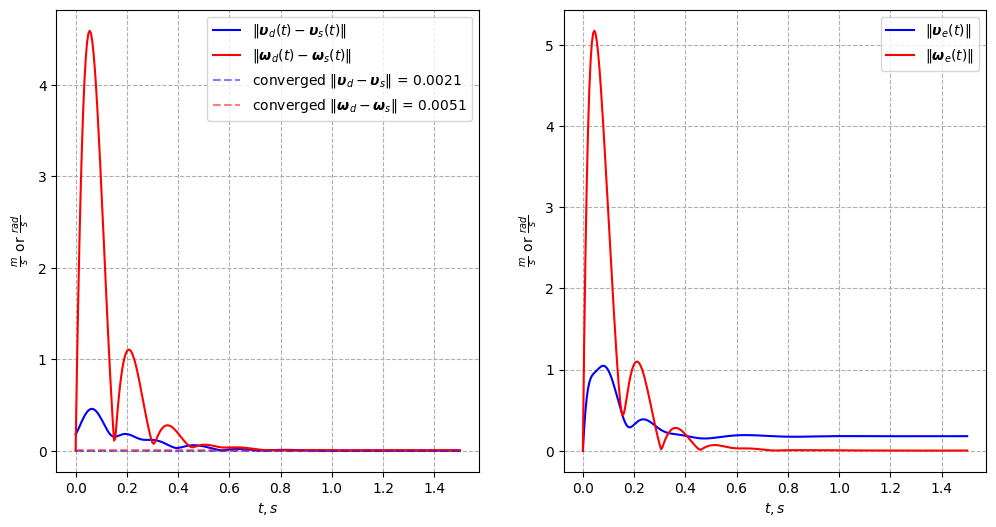
\includegraphics[scale=0.52]{figs/vels_history.png}
    \caption{Experimental frame velocities}
    \label{fig:vels_plot}
\end{figure}

The graph of difference between desired position and actual one converges to 
zero with some numerical noise. In Fig. \ref{fig:poses_plot} the obtained 
values are mean after $t > 1.5$. The steady state response time is less 
than $0.75$ second according to Fig. \ref{fig:vels_plot}. Futhermore, 
the $\mathbf{e}_{\SE}$ for constraint converges faster, see  
Fig. \ref{fig:errors_plot}. However, control error converges to zero 
same as velocities.

\begin{figure}[H]
    \centering
    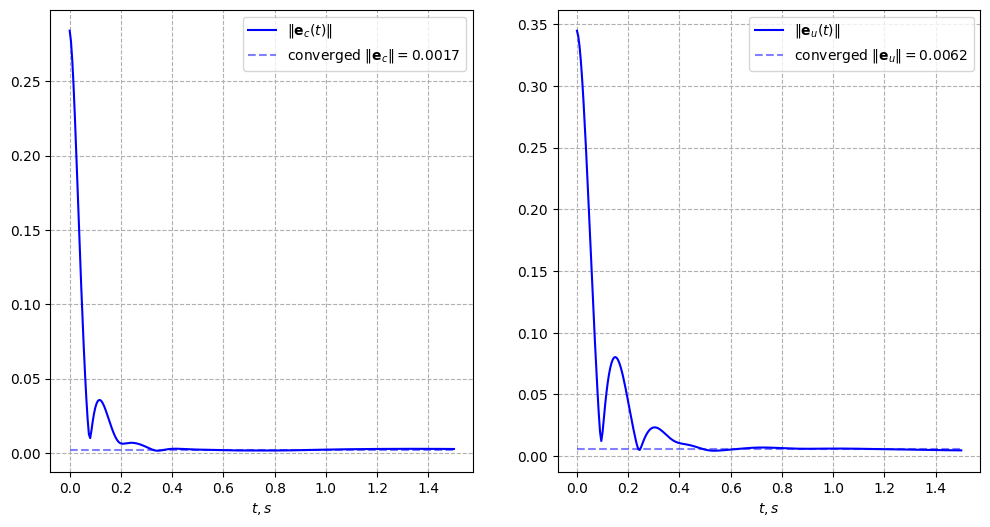
\includegraphics[scale=0.52]{figs/errors_history.png}
    \caption{Experimental $\mathbf{e}_{\SE}$, left $\mathbf{e}_c$ - constraint, 
    right $\mathbf{e}_u$ - control}
    \label{fig:errors_plot}
\end{figure}

The obtained results of numerical experiment proves the workability 
of suggested methodology. Nevertheless, results demonstrate convergence 
of over-damped system. Thus, finetuning of $K_p$, $K_d$ is still needs 
further investigations.
